\documentclass[12pt]{article}

\usepackage{amsmath, amssymb, amsthm}
\usepackage{geometry}
\usepackage{hyperref}
\usepackage{booktabs}
\usepackage{array}
\usepackage{parskip}
\usepackage{xcolor}
\usepackage{titlesec}
\usepackage{graphicx}
\usepackage{caption}
\graphicspath{{./}}

\geometry{margin=1.2in}

\title{\textbf{A Generalized Model of Community Curation Pipelines}\\[0.4em]
\large Formal Specification v1.0}
\author{Corey Petty}
\date{\today}

\newtheorem{definition}{Definition}
\newtheorem{proposition}{Proposition}
\newtheorem{remark}{Remark}

\begin{document}

\maketitle
\tableofcontents
\newpage

% ============================================================
\section{Motivation}

Social platforms face a fundamental coordination problem: content quality is unobservable at publication time, yet consumers need high-quality content to surface quickly. Traditional solutions---editorial curation, engagement algorithms, follower graphs---either centralize judgment or optimize for engagement proxies that diverge from quality.

This document formalizes a \textbf{community curation pipeline}: a market mechanism in which agents voluntarily stake resources on content signals, earning rewards proportional to their contribution and timing. Staking simultaneously (a) compensates early discovery and (b) produces a ranked feed that consumers rely on.

The model generalizes work originally done to describe the Cent/Yours Network payout system~\cite{corpetty2016}, extending it to a 4-sided market with explicit feed mechanics, consumer surplus, and formal mechanism evaluation criteria.

% ============================================================
\section{Primitives}

\subsection{Signals}

Let $\mathcal{S} = \{S_1, S_2, \ldots\}$ be the set of \textbf{signals} (content items, claims, proposals, or any community contribution) published to the platform.

Each signal $S \in \mathcal{S}$ is characterized by:
\begin{itemize}
  \item $q(S) \in [0, 1]$ --- \textbf{true quality}, a latent variable not directly observable by any agent at publication time
  \item $\tau(S) \in \mathbb{R}_{\geq 0}$ --- \textbf{publication time}
\end{itemize}

\subsection{Agents}

The platform admits four agent roles:

\begin{center}
\begin{tabular}{>{\bfseries}l l l l}
\toprule
Role & Description & Action & Incentive \\
\midrule
Creator & Produces signal $S$ & Publish & Maximize downstream revenue \\
Curator & Evaluates and endorses $S$ & Stake $v_i$ at time $t_i$ & Earn from subsequent staking \\
Consumer & Discovers and consumes $S$ & Browse ranked feed & Minimize search cost; maximize quality \\
Platform & Coordinates the market & Rank feed; extract cut & Sustain operations \\
\bottomrule
\end{tabular}
\end{center}

Let $\mathcal{C}$, $\mathcal{K}$, $\mathcal{U}$, and $\mathcal{P}$ denote the sets of curators, creators, consumers, and the platform respectively. The platform is treated as the mechanism designer, not a strategic agent.

\subsection{Stake Space}

A \textbf{stake} is any scarce resource that can be committed irrevocably to a signal. In the original Cent model this is currency; in the general case it may be tokens, reputation points, attention, or votes. We assume stakes are cardinal and summable.

% ============================================================
\section{The Staking Game}

\subsection{Setup}

Fix a signal $S$. Curators arrive and stake sequentially. Let the ordered staking sequence be:
\[
  (v_1, t_1),\ (v_2, t_2),\ \ldots,\ (v_n, t_n) \quad \text{with } t_1 < t_2 < \cdots < t_n
\]
where $v_i > 0$ is the stake of the $i$-th curator and $t_i$ is their arrival time.

\begin{definition}[Cumulative Pool]
The \textbf{cumulative pool} just before curator $i$ arrives is:
\[
  V_i^- = \sum_{k=1}^{i-1} v_k, \qquad V_1^- = 0
\]
The total pool after all $n$ curators have staked is $V_n = \sum_{k=1}^{n} v_k$.
\end{definition}

\begin{definition}[Proportional Share]
Curator $i$'s \textbf{proportional share} of the pool at the moment they stake is:
\[
  s_i = \frac{v_i}{V_i^- + v_i} = \frac{v_i}{V_{i+1}^-}
\]
For $i = 1$, the first curator holds 100\% of the pool at entry, but their share dilutes as subsequent curators arrive.
\end{definition}

\subsection{Payout Parameters}

Let $\alpha, \beta \in (0,1)$ with $\alpha + \beta < 1$. Define:
\begin{itemize}
  \item $\alpha$ --- \textbf{curator pool share}: fraction of each new stake redistributed to prior curators
  \item $\beta$ --- \textbf{platform share}: fraction taken by the platform
  \item $\gamma = 1 - \alpha - \beta$ --- \textbf{creator share}: remainder going to the content creator
\end{itemize}

\subsection{Payout Function}

\begin{definition}[Individual Payout]
When curator $j$ stakes $v_j$, the \textbf{payout to prior curator} $i < j$ is:
\[
  \pi(i,j) = v_j \cdot \alpha \cdot \frac{v_i}{V_j^-}
\]
\end{definition}

\begin{definition}[Total Curator Earnings]
The \textbf{total earnings} of curator $i$ over the lifetime of signal $S$ are:
\[
  E_i = \sum_{j=i+1}^{n} \pi(i,j) = \alpha \cdot v_i \sum_{j=i+1}^{n} \frac{v_j}{V_j^-}
\]
\end{definition}

\begin{remark}
The inner sum $\Phi_i = \sum_{j=i+1}^{n} \frac{v_j}{V_j^-}$ measures the \emph{relative growth} of the pool after curator $i$ arrived. Earlier curators face a smaller denominator $V_j^-$ for each subsequent $j$, yielding larger $\Phi_i$. This is the formal expression of the first-mover advantage. Figure~\ref{fig:bubble} illustrates this empirically: under a mixed-normal stake distribution, early-arriving curators are overwhelmingly profitable regardless of stake size. Figure~\ref{fig:earnings_trajectory} traces the earnings accumulation trajectory for individual curators, making the divergence between early and late arrivals concrete.
\end{remark}

\begin{figure}[h]
  \centering
  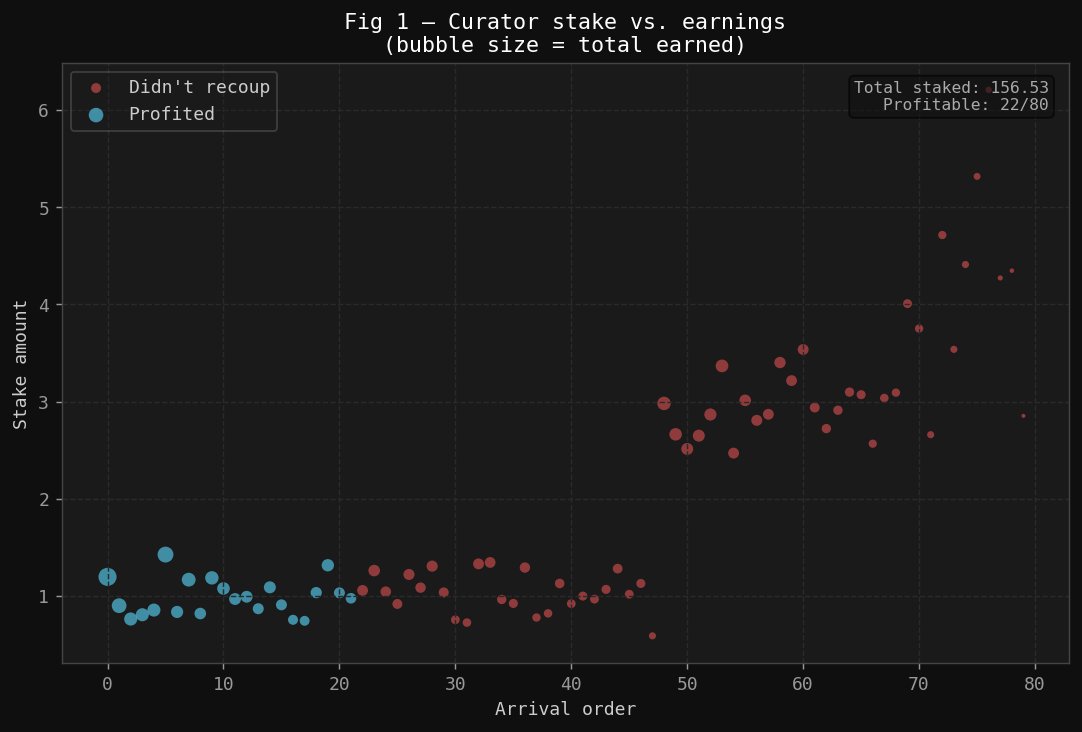
\includegraphics[width=0.92\linewidth]{fig1_bubble.png}
  \caption{Curator stake vs.\ total earnings (mixed-normal stake distribution, $\alpha=0.5$, $n=80$). Bubble size encodes total earnings; blue = profitable (recouped stake), red = did not recoup. Curators who arrived early are predominantly profitable regardless of stake magnitude.}
  \label{fig:bubble}
\end{figure}

\begin{figure}[h]
  \centering
  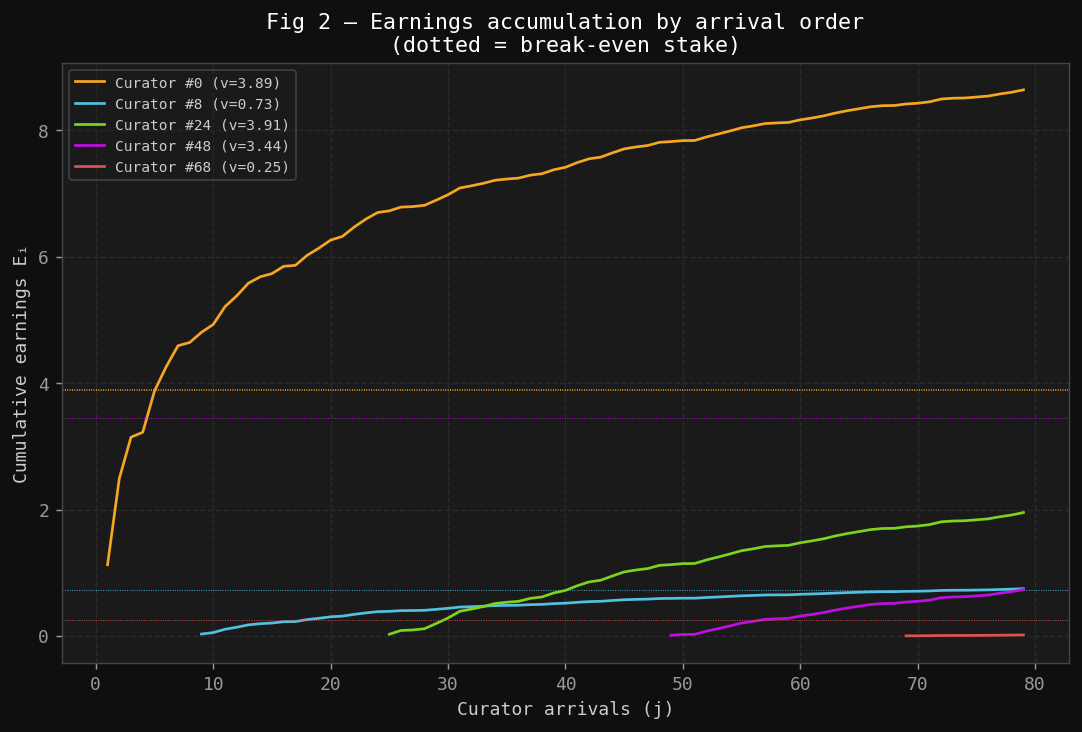
\includegraphics[width=0.92\linewidth]{fig2_earnings_trajectory.png}
  \caption{Cumulative earnings $E_i$ as a function of subsequent curator arrivals for five representative curators (uniform stake distribution, $\alpha=0.5$). Dotted horizontal lines mark each curator's break-even stake. The earliest curator (orange) captures a disproportionate share of every subsequent stake.}
  \label{fig:earnings_trajectory}
\end{figure}

\subsection{Revenue by Role}

The three-way split between curators, creator, and platform is governed by $\alpha$, $\beta$, and $\gamma$. Figure~\ref{fig:revenue_split} sweeps $\alpha$ across the feasible range to show how this tradeoff plays out in practice.

\textbf{Platform revenue:}
\[
  \Pi_{\mathcal{P}} = \beta \cdot V_n
\]

\textbf{Creator revenue:}
\[
  \Pi_{\mathcal{K}} = v_1(1 - \beta) + \sum_{j=2}^{n} v_j \cdot \gamma
\]
(The first curator's stake flows entirely to the creator minus the platform cut; subsequent stakes split three ways.)

\textbf{Total curator revenue:}
\[
  \Pi_{\mathcal{C}} = \alpha \cdot (V_n - v_1)
\]

\begin{proposition}[Conservation]
All stake is accounted for:
\[
  \Pi_{\mathcal{P}} + \Pi_{\mathcal{K}} + \Pi_{\mathcal{C}} = V_n
\]
\end{proposition}

\begin{figure}[h]
  \centering
  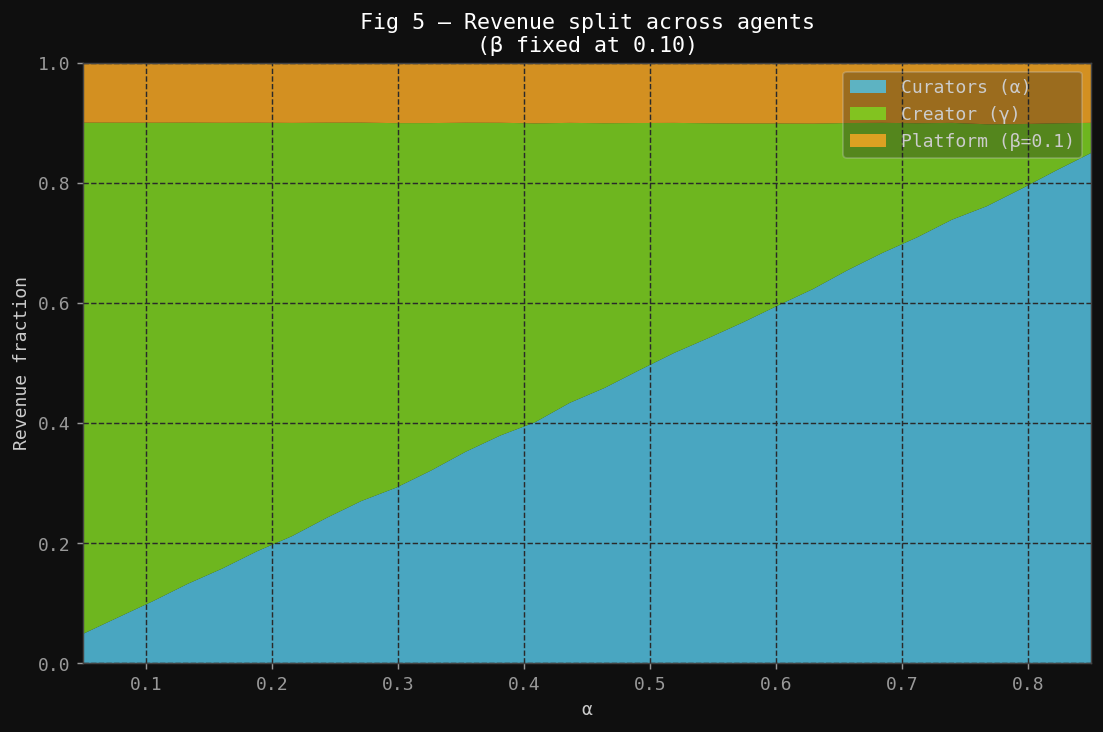
\includegraphics[width=0.92\linewidth]{fig5_revenue_split.png}
  \caption{Stacked revenue fractions for each agent class as $\alpha$ varies ($\beta=0.10$ fixed, $n=60$). At $\alpha \approx 0.45$ curators and creator receive roughly equal shares of non-platform revenue. Increasing $\alpha$ above $\sim$0.7 substantially compresses creator revenue.}
  \label{fig:revenue_split}
\end{figure}

% ============================================================
\section{Feed Mechanics}

\subsection{Ranking Function}

\begin{definition}[Rank Score]
The \textbf{rank score} of signal $S$ at time $t$ is:
\[
  R(S, t) = \sum_{i:\, t_i \leq t} w(t - t_i) \cdot v_i
\]
where $w : \mathbb{R}_{\geq 0} \to \mathbb{R}_{> 0}$ is a \textbf{temporal weight function}.
\end{definition}

The consumer feed at time $t$ is the ordered list of signals in $\mathcal{S}$ sorted by $R(S, t)$ descending. Feed position is thus a direct function of collective curator behavior.

\subsection{Temporal Weight Functions}

Four natural choices for $w(\Delta t)$:

\begin{center}
\begin{tabular}{l l l}
\toprule
Name & $w(\Delta t)$ & Behavior \\
\midrule
Accumulation & $1$ & Pure stake total; no recency bias \\
Exponential decay & $e^{-\lambda \Delta t}$ & Recent stakes dominate; $\lambda$ is half-life parameter \\
Power law & $(1 + \Delta t)^{-\theta}$ & Heavy-tailed; HN-style algorithm \\
Step window & $\mathbf{1}[\Delta t \leq W]$ & Only stakes within last $W$ time units count \\
\bottomrule
\end{tabular}
\end{center}

\begin{remark}
The choice of $w(\cdot)$ creates a tension between \emph{stability} (rewarding proven quality) and \emph{freshness} (surfacing new content). Figure~\ref{fig:ranking_decay} compares all four weight functions on the same staking sequence: the accumulation function never decays, permanently advantaging old staked content; time-decay variants restore freshness at the cost of rank stability. A key empirical question is which weight function best predicts consumer satisfaction.
\end{remark}

\begin{figure}[h]
  \centering
  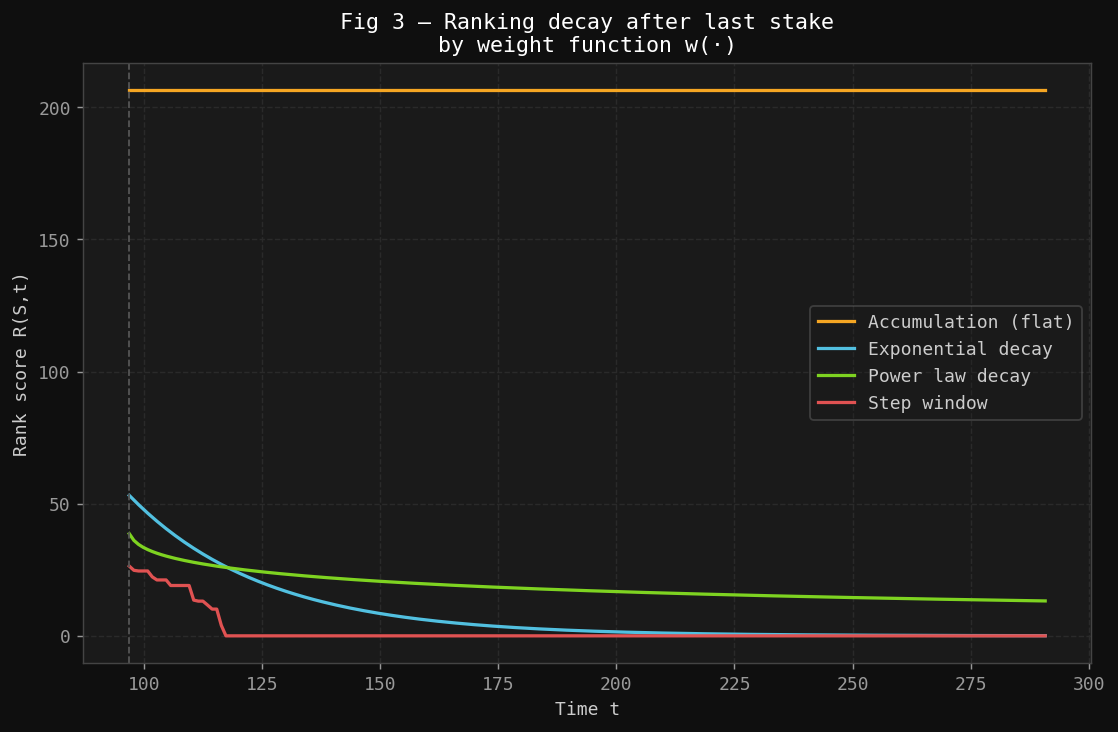
\includegraphics[width=0.92\linewidth]{fig3_ranking_decay.png}
  \caption{Rank score $R(S,t)$ under four weight functions after staking stops (dashed vertical). Accumulation rank never decays, allowing old content to permanently dominate the feed. Exponential and power-law decay gracefully derank stale content; the step window hard-resets at boundary $W$.}
  \label{fig:ranking_decay}
\end{figure}

\subsection{The Staking--Feed Duality}

A central structural observation: \textbf{the curator payout function and the consumer feed ranking are the same data structure viewed from different perspectives}. The staking pool $\{(v_i, t_i)\}$ simultaneously:
\begin{enumerate}
  \item Determines curator earnings via $E_i$
  \item Determines signal rank via $R(S, t)$
\end{enumerate}

This means incentive design and feed quality are coupled. You cannot change one without affecting the other.

% ============================================================
\section{Consumer Surplus}

\subsection{Individual Utility}

Consumer $u$ visiting the feed at time $t$ receives utility from consuming signal $S$ at rank position $r(S, t)$:
\[
  U_u(S, t) = q(S) - c(r(S, t))
\]
where $c : \mathbb{N} \to \mathbb{R}_{\geq 0}$ is an increasing \textbf{search cost function}. Natural choices include $c(r) = \kappa \log r$ or $c(r) = \kappa / r^{-1}$.

\subsection{Aggregate Consumer Surplus}

\[
  CS(t) = \sum_{u \in \mathcal{U}} \sum_{S \in \mathcal{S}} \mathbf{1}[u \text{ consumes } S] \cdot U_u(S, t)
\]

A \textbf{well-functioning mechanism} maximizes $CS(t)$: high-$q$ signals rank high, low-$q$ signals sink regardless of stake concentration.

% ============================================================
\section{Mechanism Quality Metrics}

These are the primary empirical targets for validation.

\subsection{Signal Accuracy}

\begin{definition}[Signal Accuracy]
At time $t$, \textbf{signal accuracy} is the Spearman rank correlation between total stake and true quality across all signals published before $t$:
\[
  \rho(t) = \text{Corr}_{\text{Spearman}}\!\left(V_n(S),\, q(S)\right)_{S:\, \tau(S) \leq t}
\]
\end{definition}

A mechanism with $\rho(t) \to 1$ perfectly ranks by quality. $\rho(t) \approx 0$ means staking is uninformative.

\subsection{Discovery Speed}

\begin{definition}[Discovery Speed]
For a signal $S$ and threshold rank $k$, the \textbf{discovery time} is:
\[
  \Delta\tau^*(S, k) = \inf\!\left\{t : r(S, t) \leq k\right\} - \tau(S)
\]
\end{definition}

A lower $\Delta\tau^*$ for high-$q$ signals is desirable. Ideally, discovery time is negatively correlated with quality. Figure~\ref{fig:discovery} traces a single content item's rank trajectory as curators arrive in real time, marking the moment it crosses the consumer discovery threshold and showing how weight function choice affects both when that crossing occurs and whether the item later recedes to make room for fresher content.

\begin{figure}[h]
  \centering
  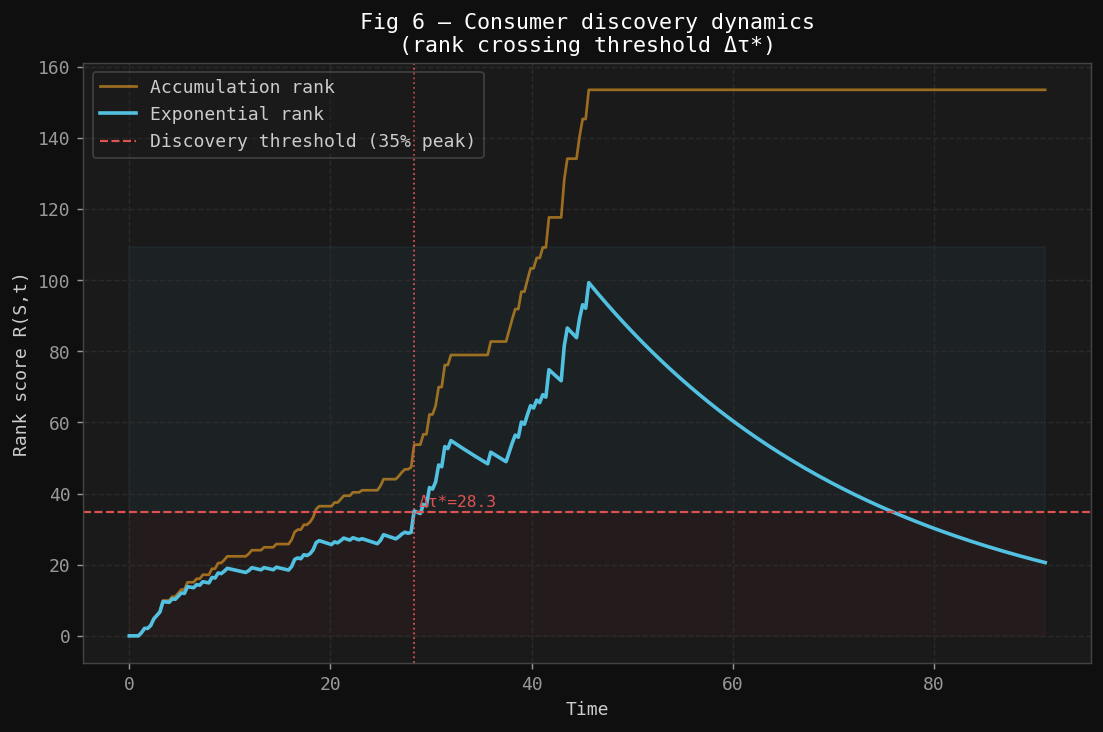
\includegraphics[width=0.92\linewidth]{fig6_discovery.png}
  \caption{Rank score rising as curators arrive (exponential inter-arrival times). The red dashed line marks the consumer discovery threshold; content becomes visible in the feed at $\Delta\tau^*$. Exponential-decay rank (blue) peaks and then naturally recedes as the content ages; accumulation rank (gold) never falls.}
  \label{fig:discovery}
\end{figure}

\subsection{Curator ROI}

\begin{definition}[Curator ROI]
The \textbf{return on investment} for curator $i$ is:
\[
  \mathrm{ROI}_i = \frac{E_i - v_i}{v_i} = \frac{E_i}{v_i} - 1
\]
\end{definition}

The \textbf{participation constraint} requires $\mathbb{E}[\mathrm{ROI}_i] > 0$ for rational agents to stake. Characterizing when this holds is a key analytical target. Figure~\ref{fig:roi_phase} maps the ROI landscape across arrival fractions and $\alpha$ values: the break-even point is clearly visible, and its leftward shift as $\alpha$ decreases quantifies how much the profitable participation window shrinks under tighter curator allocations.

\begin{figure}[h]
  \centering
  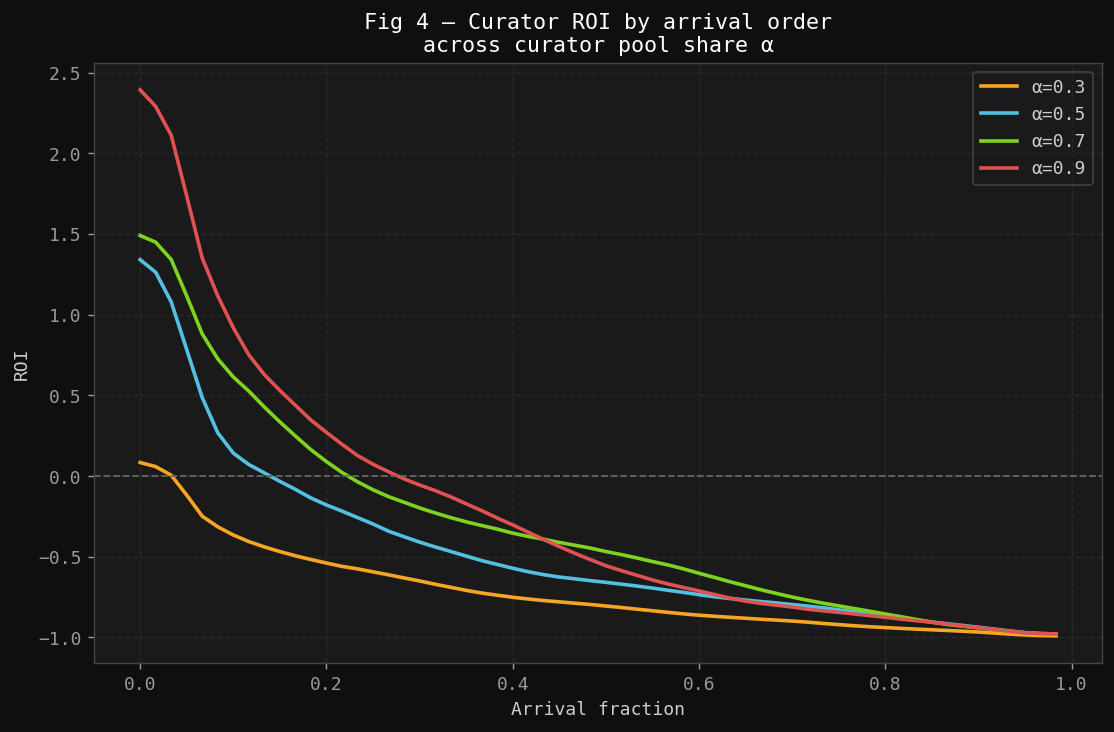
\includegraphics[width=0.92\linewidth]{fig4_roi_phase.png}
  \caption{Smoothed curator ROI as a function of arrival fraction across four values of $\alpha$ (uniform stake distribution, $n=60$). The break-even crossing (ROI = 0) shifts leftward as $\alpha$ decreases, shrinking the profitable participation window. Higher $\alpha$ is necessary but not sufficient for broad curator participation.}
  \label{fig:roi_phase}
\end{figure}

% ============================================================
\section{Open Questions for Validation}

\subsection{Analytical Questions}

\begin{enumerate}
  \item \textbf{Participation constraint}: For what distributions of $\{v_j\}_{j>i}$ and total $n$ does $\mathbb{E}[E_i] > v_i$? Is there a closed-form threshold?

  \item \textbf{Equilibrium timing}: Is there a Nash equilibrium in the timing game? Does the first-mover advantage create a race to stake immediately, or does strategic delay emerge (wait to see if others validate first)?

  \item \textbf{Optimal weight function}: Which $w(\cdot)$ maximizes $\rho(t)$ under a given stake distribution?

  \item \textbf{Mechanism robustness}: If a coordinated coalition of size $m$ stakes each other's low-quality content, how much does $\rho(t)$ degrade? What minimum honest participation is needed for accuracy?
\end{enumerate}

\subsection{Simulation Questions}

\begin{enumerate}
  \item How do curator earnings differ under uniform vs.\ power-law stake distributions?
  \item How does the choice of $\alpha$ affect feed accuracy vs.\ curator participation rate?
  \item What is the effect of a time-decay weight $w(\cdot)$ on the stability of the feed ranking?
\end{enumerate}

\subsection{Empirical Questions}

\begin{enumerate}
  \item On real platforms (Reddit, Hacker News, Mirror, Sound.xyz), does early endorsement predict final quality as measured by external signals?
  \item Is curator ROI positive in expectation on platforms with explicit curator rewards?
  \item Do platforms with time-decay ranking produce feeds with higher measured consumer satisfaction than pure accumulation platforms?
\end{enumerate}

% ============================================================
\section{Proposed Research Plan}

\begin{enumerate}
  \item \textbf{Analytical}: Derive closed-form participation constraints; characterize Nash equilibria in timing game (Section 6.1)
  \item \textbf{Simulation}: Extend the original \texttt{cent\_modeling} codebase with:
    \begin{itemize}
      \item Configurable weight functions $w(\cdot)$
      \item Multiple stake distributions
      \item Coalition attack scenarios
      \item Metrics: $\rho(t)$, $\Delta\tau^*$, $\mathrm{ROI}_i$ across parameter sweeps
    \end{itemize}
  \item \textbf{Empirical}: Collect and analyze data from platforms with public APIs (Reddit, HN, Mirror) to validate model predictions
  \item \textbf{Write-up}: Generalized model paper; compare to TCR, bonding curve, and prediction market literature
\end{enumerate}

% ============================================================
\begin{thebibliography}{9}

\bibitem{corpetty2016}
Petty, C. (2016). \textit{cent\_modeling: Modeling Cent.co Payout System}. GitHub.
\url{https://github.com/corpetty/cent_modeling}

\end{thebibliography}

\end{document}
